\documentclass[class=report,crop=false, 12pt]{standalone}
\usepackage[screen]{../myscratch}

\begin{document}


\titre[E]{Répéter}
%===============================

\begin{enigme}
\sauteligne

\begin{center}
  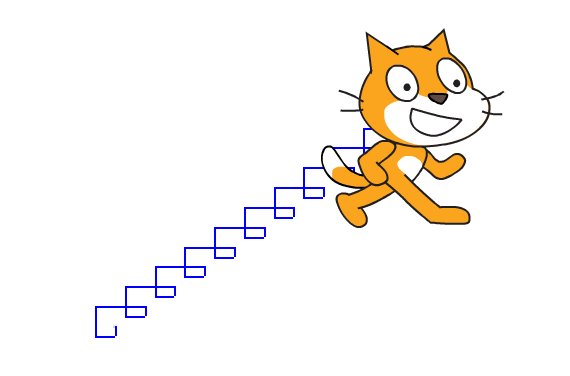
\includegraphics[width=0.5\textwidth]{ecran-02-eg1}
\end{center}

Scratch se place en $x=0$ et $y=0$ et répète ensuite 10 fois les instructions suivantes :
\begin{itemize}
  \item s’orienter à $180$\textdegree
  \item avancer de $5$
  \item s’orienter à $-90$\textdegree 
  \item avancer de $10$
  \item s’orienter à $0$\textdegree
  \item avancer de $15$
  \item s’orienter à $90$\textdegree
  \item avancer de $25$
\end{itemize}

\bigskip

\textbf{Question.} À la fin, quelle est la position de Scratch ? Quelle est la valeur de l'abscisse $x$ ? Quelle est la valeur de l'ordonnée $y$ ? 

%\begin{solution}
%Réponse : $x=150$, $y = 100$.
%\end{solution}

\end{enigme}



\begin{enigme}
On considère les instructions suivantes :
\begin{itemize}
  \item avancer de 20
  \item tourner vers la gauche de 15 degrés
\end{itemize}

\bigskip

\textbf{Question.} Combien de fois faut-il répéter ces deux instructions pour revenir à la position de départ ? 

%\begin{solution}
%Réponse : $360/15 = 24$ côtés.
%\end{solution}

\end{enigme}


\begin{enigme}
Le code suivant affiche un carré avec des pointes triangulaires sur chaque côté. 


\bigskip

\begin{center}
\begin{scratch}
  \blockinit{quand \greenflag est cliqué}
  \blockmove{aller à x: \ovalnum{0} y: \ovalnum{0}}
  \blockmove{s'orienter à \ovalnum{90}}
  \blockpen{effacer tout}
  \blockpen{stylo en position d'écriture}
  \blocklook{montrer}
  \blockrepeat{répéter \ovalnum{4} fois}
  {
    \blockrepeat{répéter \ovalnum{3} fois}
    {
      \blockmove{avancer de \ovalnum{20} pas} 
      \blockmove{tourner \turnright{} de \ovalnum{60} degrés}
      \blockmove{avancer de \ovalnum{10} pas} 
      \blockmove{tourner \turnleft{} de \ovalnum{120} degrés}
      \blockmove{avancer de \ovalnum{10} pas} 
      \blockmove{tourner \turnright{} de \ovalnum{60} degrés}
      \blockmove{avancer de \ovalnum{20} pas} 
    }
  \blockmove{tourner \turnleft{} de \ovalnum{90} degrés}
  }
  \blocklook{cacher}
\end{scratch}
\end{center} 

\bigskip

\textbf{Question.} Combien y a-t-il de petites pointes triangulaires en tout ? 
%\begin{solution}
%Réponse : $4 \times 3 = 12$ triangles.
%\end{solution}

\end{enigme}


\end{document}


